\documentclass[border=4pt]{standalone}
\usepackage{pgfplots}
\usepgfplotslibrary{groupplots}
\usetikzlibrary{calc}
\pgfplotsset{compat=1.18}
\begin{document}
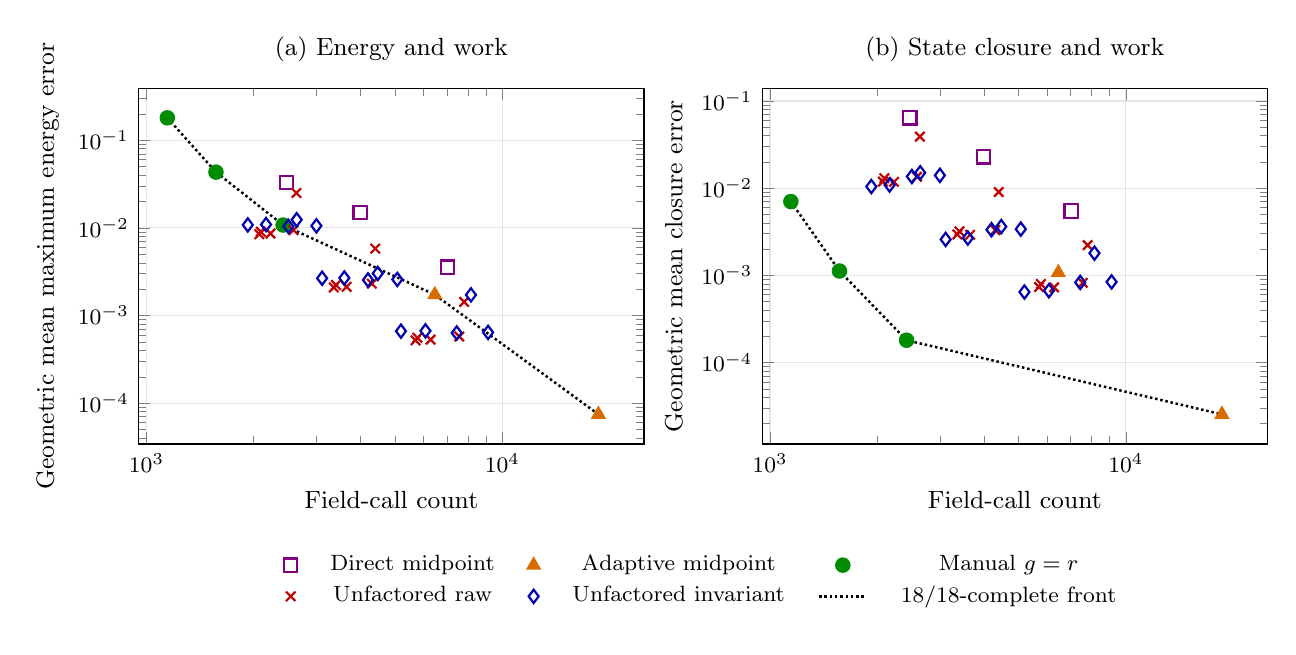
\begin{tikzpicture}
\begin{groupplot}[group style={group size=2 by 1,horizontal sep=1.5cm,group name=costgrid},
width=8cm,height=6.1cm,xmode=log,ymode=log,grid=major,grid style={gray!20},
xlabel={Field-call count},label style={font=\small},tick label style={font=\footnotesize},
title style={font=\small},xmin=950,xmax=25000,legend columns=3,
legend style={draw=none,font=\footnotesize,column sep=0.35cm}]
\nextgroupplot[title={(a) Energy and work},ylabel={Geometric mean maximum energy error},legend to name=costlegend]
\addplot+[only marks,mark=square,color=violet,mark size=2.4pt,mark options={solid,line width=0.8pt}] coordinates {(2472.421004651,0.03280178775347) (3981.688191838,0.0149790791346) (7015.531782418,0.003571359188067)};
\addlegendentry{Direct midpoint}
\addplot+[only marks,mark=triangle*,color=orange!85!black,mark size=2.4pt,mark options={solid,line width=0.8pt}] coordinates {(6458.553044823,0.001729880644941) (18617.38443497,7.463066371123e-05)};
\addlegendentry{Adaptive midpoint}
\addplot+[only marks,mark=*,color=green!55!black,mark size=2.4pt,mark options={solid,line width=0.8pt}] coordinates {(1144.224268136,0.1802210507826) (1567.460664716,0.04328953781721) (2419.861334701,0.01077768560971)};
\addlegendentry{Manual $g=r$}
\addplot+[only marks,mark=x,color=red!75!black,mark size=2.4pt,mark options={solid,line width=0.8pt}] coordinates {(2075.315772031,0.00847099971401) (3359.903519486,0.002091751339733) (5701.241332705,0.0005207898487295) (2588.298191248,0.009429152051747) (4296.351156734,0.002311680934177) (7569.49793034,0.0005763393575703) (2230.158401456,0.008628536036127) (3649.775600741,0.002128931903644) (6284.296929446,0.0005309241299737) (2095.564050665,0.009051538812968) (3407.102199873,0.002234266437301) (5769.233319272,0.0005578204200052) (2637.226707594,0.02502977397422) (4392.073139952,0.005799331662819) (7808.414512738,0.001431848529384)};
\addlegendentry{Unfactored raw}
\addplot+[only marks,mark=diamond,color=blue!70!black,mark size=2.4pt,mark options={solid,line width=0.8pt}] coordinates {(1925.908301255,0.01081525668942) (3115.183426537,0.002663466141144) (5187.50797318,0.0006637771254895) (3001.618734938,0.01056350940844) (5066.125194264,0.002581118649875) (9116.223777589,0.0006417633948022) (2504.154111689,0.0104163757478) (4191.419660802,0.00254543446903) (7442.88372425,0.0006326873655846) (2642.412880426,0.0123996189661) (4464.483593879,0.003023730727402) (8159.955137155,0.001720237750663) (2167.413458178,0.01092778781709) (3596.505506212,0.002682426289581) (6078.87650816,0.0006687311222363)};
\addlegendentry{Unfactored invariant}
\addplot+[black,densely dotted,mark=none,line width=0.9pt] coordinates {(1144.224268136,0.1802210507826) (1567.460664716,0.04328953781721) (2419.861334701,0.01077768560971) (6458.553044823,0.001729880644941) (18617.38443497,7.463066371123e-05)};
\addlegendentry{18/18-complete front}
\nextgroupplot[title={(b) State closure and work},ylabel={Geometric mean closure error}]
\addplot+[only marks,mark=square,color=violet,mark size=2.4pt,mark options={solid,line width=0.8pt}] coordinates {(2472.421004651,0.06406491619928) (3981.688191838,0.02286140494676) (7015.531782418,0.005476821761045)};
\addplot+[only marks,mark=triangle*,color=orange!85!black,mark size=2.4pt,mark options={solid,line width=0.8pt}] coordinates {(6458.553044823,0.001077979214667) (18617.38443497,2.548633987403e-05)};
\addplot+[only marks,mark=*,color=green!55!black,mark size=2.4pt,mark options={solid,line width=0.8pt}] coordinates {(1144.224268136,0.007019393573266) (1567.460664716,0.001121745771505) (2419.861334701,0.0001805028106366)};
\addplot+[only marks,mark=x,color=red!75!black,mark size=2.4pt,mark options={solid,line width=0.8pt}] coordinates {(2075.315772031,0.01188905661775) (3359.903519486,0.002942824748987) (5701.241332705,0.0007338145926719) (2588.298191248,0.0135108873353) (4296.351156734,0.003306626140194) (7569.49793034,0.0008224495360867) (2230.158401456,0.0118215679755) (3649.775600741,0.002921644434672) (6284.296929446,0.0007282862988407) (2095.564050665,0.01300691649339) (3407.102199873,0.003200949341998) (5769.233319272,0.000797146204487) (2637.226707594,0.03898476313027) (4392.073139952,0.00903852865652) (7808.414512738,0.002224519307707)};
\addplot+[only marks,mark=diamond,color=blue!70!black,mark size=2.4pt,mark options={solid,line width=0.8pt}] coordinates {(1925.908301255,0.0104331162461) (3115.183426537,0.002583392763037) (5187.50797318,0.0006442885269456) (3001.618734938,0.01403002026892) (5066.125194264,0.003390907987297) (9116.223777589,0.0008414442732228) (2504.154111689,0.01360684381081) (4191.419660802,0.003337342647601) (7442.88372425,0.0008303687021244) (2642.412880426,0.01502537240054) (4464.483593879,0.003623444656619) (8159.955137155,0.00179716654579) (2167.413458178,0.01086684710797) (3596.505506212,0.002676869101923) (6078.87650816,0.0006667671029991)};
\addplot+[black,densely dotted,mark=none,line width=0.9pt] coordinates {(1144.224268136,0.007019393573266) (1567.460664716,0.001121745771505) (2419.861334701,0.0001805028106366) (18617.38443497,2.548633987403e-05)};
\end{groupplot}
\node[anchor=north] at ($(costgrid c1r1.south)!0.5!(costgrid c2r1.south)+(0,-1.15cm)$) {\pgfplotslegendfromname{costlegend}};
\end{tikzpicture}
\end{document}
